\subsection{Training}
For now, the current training procedure is:

\begin{enumerate}
	\item[1.] Generate a large number of MAGBOX events (signal and background).
	\item[2.] Voxelize the MC truth.  The voxels need not be connected.
	\item[3.] Slice the events in slices of width $w$ using the voxelized MC truth, including all voxels in the $xy$ plane with $z$ in the range of the slice $(z_i, z_i + w)$.  Each slice is then a 2D grid (with pixel dimensions equal to those of the voxel $xy$ dimensions) containing some energy.  If any slice in the event has an $xy$ range greater than some value, or if more $z$ slices than some limit are present, do not include any slices from the event in the training set.
	\item[4.] For each slice, normalize the total energy to 1, and for each pixel in the slice containing nonzero energy, cast EL light on an $M \times M$ SiPM plane (M to be chosen appropriately, currently $M = 20$) using the S2 parameterization.  This SiPM map along with the true slice information constitutes the input and truth for a single training event.
	\item[5.] Train the net on the constructed slices.  Using a softmax output layer, the reconstructed projection will provide a normalized image of the track.
\end{enumerate}

\noindent An example of a training event (truth, SiPM map, and reconstructed slice) is shown in figure \ref{fig:slice_train}.

\begin{figure}[!htb]
	\centering
	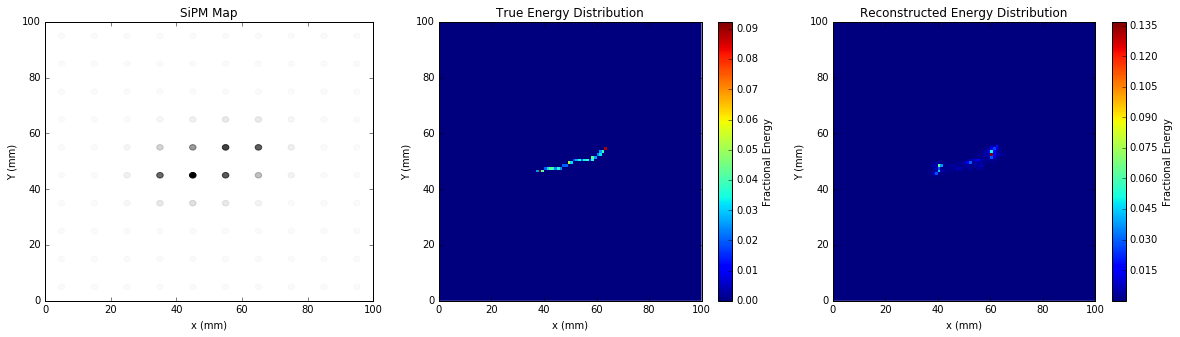
\includegraphics[scale=0.41]{fig/reconst_example_evt1.png}
	\caption{\label{fig:slice_train}Example of reconstruction of a single slice. The normalized SiPM map (left) produced by the true energy distribution (middle), as reconstructed by a simple CNN (right).}
\end{figure}